%!TEX root = ../thesis.tex
%*******************************************************************************
%*********************************** Third Chapter *****************************
%*******************************************************************************

\chapter{Implementation and methods}  %Title 

\ifpdf
    \graphicspath{{Chapters/Chapter3/Figs/Raster/}{Chapters/Chapter3/Figs/PDF/}{Chapters/Chapter3/Figs/}}
\else
    \graphicspath{{Chapters/Chapter3/Figs/Vector/}{Chapters/Chapter3/Figs/}}
\fi


%********************************** %First Section  **************************************
\section{Building a structured library of abstractions}

BeesBook is well-suited for testing a broad range of hypotheses % no existing hyp atm
on the data it collects. This work attempts to use BeesBook’s data
to pinpoint the moment in which workers transition to foraging, and potentially
answer some questions about the circumstances of that transition. 

I propose an approach of defining abstractions layered on top of the original
form of the data (which is a list of detections). Each abstraction is conceived
as a step in a funnel that starts with detections and is meant to produce the
status of being a forager (or not).

\begin{figure}[htbp!] 
\centering    
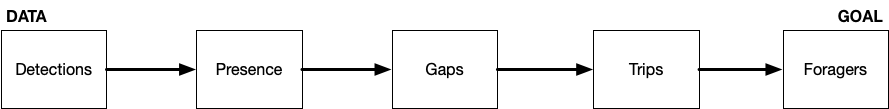
\includegraphics[width=1.0\textwidth]{basic_funnel}
\caption[basic-funnel]{Visualization of the abstraction steps}
\label{fig:basic_funnel}
\end{figure}


On top of Detections, I define Presence as a numerical score equal to the
number of Detections that were registered for a given bee in a time window of
$t=30$ seconds. On top of Presence, I define Gaps as periods of time where bees
had a Presence score of zero or close. On top of that, I define Trips as Gaps that
seem to be caused by the bee leaving the hive (as opposed to occlusion, entering
brood cells etc.). I finally want to use Trips as a metric that lets us determine when
a given bee has started to forage. A more detailed description of the process,
along with a list of potential problems, is presented below.

The first key idea is the ability to reuse such abstractions for work with
other research goals. For example, (Marcus, 2019) examines the deaths of bees %TODO: cite Marcus 
(and their potential reasons) using Presence. 
For research into other parts of the DOL or related in-hive
behavior, the first three abstractions could be reused (e.g. Gaps
for an investigation into behavior that relates to cleaning brood cells). 

The second key idea is to apply the same methodology for all new research goals.
If existing abstractions cannot be reused, defining new ones in a preservable or 
reproducible way ensures future analyses will be much easier to perform.  

%TODO: illustration: abstraction graph


%********************************** %Second Section  **************************************
\section{Detections to Presence}
A Detection in the BeesBook database is the result of a single bee tag being
recognized in a single frame of video. If that tag is also visible in the next
frame, this is registered as a new detection. Each detection has information on
where the tag was detected (x/y coordinates and orientation), when (exact
timestamp), with what confidence and by which of the four cameras. 

TODO: TABLE: an example detection

Calculating Presence scores from raw detections is tallying up the number of
times a given bee was detected in a 30-sec interval window. The interval size
was chosen arbitrarily, albeit with some experimentation. The code was written
in a way that allows for easy re-generation of Presence scores with a different
interval window size. Another important hyperparameter is the confidence
requirement. Every detection has a confidence value assigned to it, representing
the likelihood that the tag was decoded properly (i.e. belongs to the bee it was
assigned to, and not another one).

Determining a good confidence requirement could conceivably have great influence
on the next steps. A very high threshold could mean that too many valid
detections are filtered out and artificial troughs in presence score are created
in consequence. A low one could mean including detections that did not really
occur (should not have occured) and artificial peaks in presence score are
created. The way the process is currently designed, it has more robustness
towards including fake detections than it has toward discarding real ones. It is
therefore reasonable to suspect a fairly low confidence rate should give better results. 
I tried thresholds of $0.2$ and $0.99$ and present the results in the Evaluation section.
The interval window has less significance and is easier to get right. If it’s small, it could
lead to unnecessary calculation, too large and it could lead to short artificial
gaps in presence. [Mention the framing of this as robustness against false
positives vs false negatives]

%TODO: FIG: distribution of confidence values in detections from e.g. one given day). 

Each camera records with a speed of 3FPS. With an interval size of 30 seconds,
that gives a max expected Presence score of 90 (with exceptions - see the Problems section below).
The score is then thresholded at X,
mapping it to a binary function. That function is smoothed out by morphological
closing with a parameter of X. 

%TODO: FIG: a day of presence, as score and as a binarized function

%TODO: stub: A big part of the purpose (advantage of PRES over DET) is reduced
%size/greater speed. Det file for 1h is 400mb, presence for a day is 12mb.


From the binarized and smoothed out form of presence, Gaps are generated by
taking the difference between Presence values for intervals i +1 and i, for all
intervals. This identifies exits (whenever the difference is -1) and entries
(whenever the difference is 1). 

This makes up a long list of all situations, where the video cameras lost track
of a bee. 

For a sample of those situations, I generate videos for manual analysis. 

Foraging trips are the single most defining aspect of the forager’s life and a
natural starting point for the investigation. No other bee caste is expected to
disappear from the cameras’ field of vision with such frequency and regularity.
We therefore decide on looking closer into trips as our primary method of
identifying foragers. We start with a raw list of detections as offered by the
BeesBook database (See the format Fig X / Appendix I). In order to convincingly
determine an absence period’s beginning and end, we divide the time of the
entire experiment into intervals of n seconds. For every such interval, we go
through all possible bee ids and mark the cell for [given interval, given
bee\_id) with a 1 if the database contains at least one detection for given bee
with a timestamp within the bounds of the given time interval. This produces a
matrix of binary values representing every bee’s history of hive presence.



Fig. X - Illustration of the presence dataframe, dark cell background meaning
present, light meaning absent. 


Given the presence matrix, we interpret a bee’s absence and reappearance as a
trip. In order to prevent misclassified detections (TODO: cite BeesBook’s
misclassification rate)  from artificially increasing the number of trips, we
smooth out the presence matrix with a rolling median (window\_size = r). This
means, that any period of presence or absence shorter than floor(r/2) will be
ignored.

We then summarize the amount of trips a given bee has taken on a given day. This
hopefully makes foragers distinct from non-foragers 

It is important to note that that when requesting data from the database, we
pass a ‘desired confidence’ value c. This value, together with the size of the
interval in seconds (n) and the size of the rolling window that smoothes out the
detections (r) are three very important hyperparameters that contribute to the
accuracy of the resulting trip data and to the credibility of conclusions we
might draw from them.  <to be continued>

Ideas: talk about false positives and false negatives with a presence map for
all bees, just take some statistical hints - %of time in hive! check
(dis)appearence proximity to exit 

\section{Known issues and approaches to addressing them}

Misidentified tags Binary tags, especially such with no error-correcting bits,
can sometimes be have a problem with misclassified (wrongly assigned) tags. In
the case of BeesBook, this effect was corrected in (Boenisch, 2018) by tracking
(combining series of detections into paths based on their locations and
timestamps). The initial ~13% of incorrect decodings was reduced to ~2%. 

Overlaps Because the field-of-view of camera 0 overlaps with camera 1 and camera
2 overlaps with camera 3, we get duplicate detections whenever a bee enters a
thin horizontal area in the middle of either sides of the hive (the overlap
areas). Those detections are still true by definition of a BeesBook detection,
but they often push the presence score above the assumed maximum of 90. This is
resolved simply by replacing any >90 score with 90. The reasoning behind this is
that a bee with duplicate detections should be considered present in the hive
(all the more given the fact that the overlap areas are not close to the hive
exit).

Camera outages On occasion, there were camera outages. This is resolved by
removing the affected days from the data. A simple figure that maps outages by
day, adapted from (Schlegel, 2017), can be found in attachments. A more
elaborate interactive visualization can be accessed at (url, thesis by
Peter..(?), 201X)


Camera hiccups In case of some outages, before they happened, the camera would
produce more frames per second than it was expected to (for a period of time).
This resulted in Presence scores often reaching multiples of 90 (180 or 270),
with a maximum of (x). In the worst case, this effect can also combine with the
overlap. The reasoning here is the same as in the case of overlaps - we consider
any score above 90 as the bee being present in the hive and replace it with a 90
to ensure compatibility with the next steps of the process. 
